%% Beispiel-Präsentation mit LaTeX Beamer im KIT-Design
%% entsprechend den Gestaltungsrichtlinien vom 1. August 2020
%%
%% Siehe https://sdqweb.ipd.kit.edu/wiki/Dokumentvorlagen

%% Beispiel-Präsentation
\documentclass[de]{sdqbeamer} 
 
%% Titelbild
\titleimage{banner_2020_kit}

%% Gruppenlogo
\grouplogo{mvmdpe} 

%% Gruppenname und Breite (Standard: 50 mm)
\groupname{DPE-MVM-CIW}
%\groupnamewidth{50mm}

% Beginn der Präsentation

\title[Develoment of a robotics lab for control theory on the example of sloshing free liquid transport]{Develoment of a robotics lab for control theory on the example of sloshing free liquid transport}
\subtitle{} 
\author[Bauer]{Kai Bauer}

\date[28.\,07.\,2025]{28. Juli 2025}

% Literatur 
 
\usepackage[citestyle=authoryear,bibstyle=numeric,hyperref,backend=biber]{biblatex}
\usepackage{tikz}
\usepackage{svg}
\usepackage{chemformula}
\usepackage{circuitikz}
\usepackage{pgfplots}
\usepackage{bm}
\usepackage{bbding}
\addbibresource{presentation.bib}
\bibhang1em


\defbeamertemplate{itemize item}{boldarrow}{\raisebox{0.3ex}{\resizebox{1.2ex}{1ex}{\textcolor{kit-green100}{\ArrowBoldRightShort}}}}


%%%%%%%%%%%%%%%%%%%%%%%%%%%%%%%%%%%%%%%%%%%%%%%%%%%%%%%%%%%%%%%%%%%%%%%%%%%%%%%%%%%%%%%%%%%%%%%%%%%%%%%%%

\begin{document}
 
%%%%%%%%%%%%%%%%%%%%%%%%%%%%%%%%%%%%%%%%%%%%%%%%%%%%%%%%%%%%%%%%%%%%%%%%%%%%%%%%%%%%%%%%%%%%%%%%%%%%%%%%%

%Titelseite
\KITtitleframe

%%%%%%%%%%%%%%%%%%%%%%%%%%%%%%%%%%%%%%%%%%%%%%%%%%%%%%%%%%%%%%%%%%%%%%%%%%%%%%%%%%%%%%%%%%%%%%%%%%%%%%%%%

%Inhaltsverzeichnis
\begin{frame}{Inhaltsverzeichnis}
\tableofcontents
\end{frame}

%%%%%%%%%%%%%%%%%%%%%%%%%%%%%%%%%%%%%%%%%%%%%%%%%%%%%%%%%%%%%%%%%%%%%%%%%%%%%%%%%%%%%%%%%%%%%%%%%%%%%%%%%

\section{Autonoumous Lab}
\begin{frame}{Autonomous Lab}
    \begin{columns}[t]
        \column{.5\textwidth}
            \begin{itemize}
                \setbeamertemplate{itemize item}[tikzarrow]
                \item automation of various (repetitive) tasks
                \item provide high precision and repeatability
                \item act in a collaborative and dynamic environment
                \item adaptability to the environment
                \linebreak
                \setbeamertemplate{itemize item}[boldarrow]
                \item \bf{Assignment of a complex task in a preexisting lab environment}
            \end{itemize}        
        \column{.5\textwidth}
            \vspace{-15pt}
            \begin{figure}
                \centering
                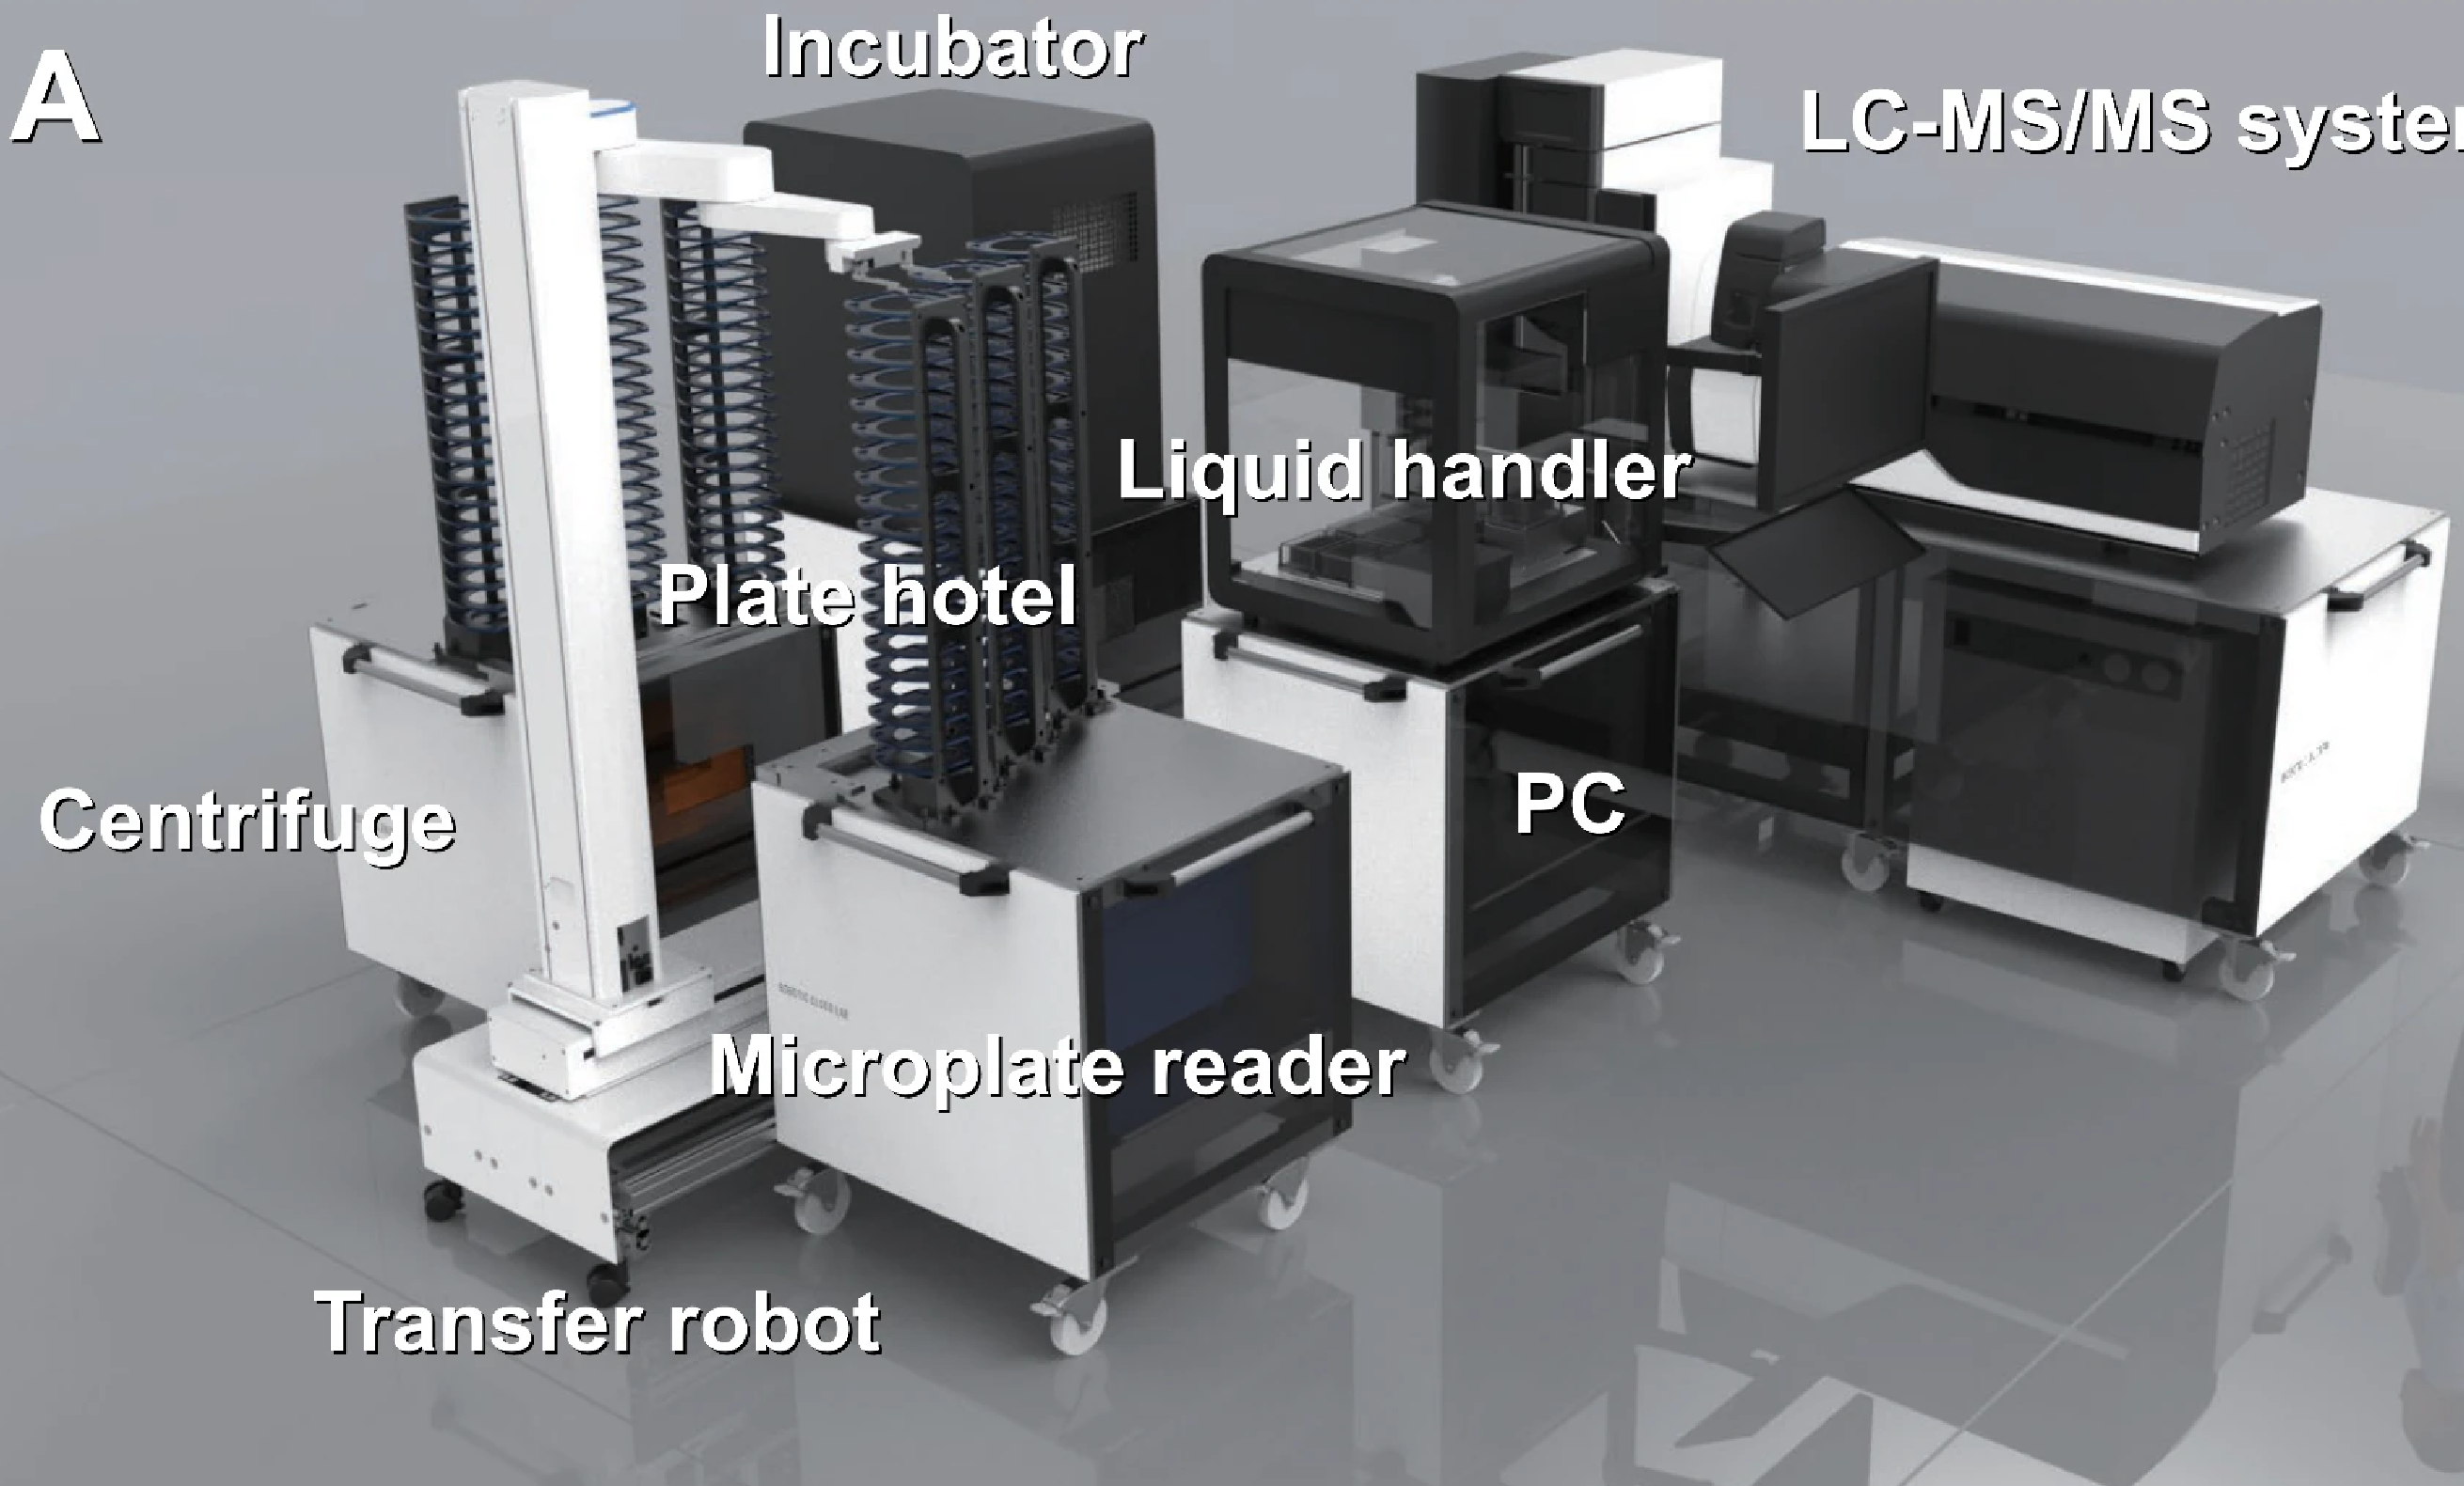
\includegraphics[scale=0.18]{graphics/stationary_lab.pdf}
                \footnotesize Robot centric autonomous lab (Fushimi, K.)
            \end{figure}
    \end{columns}
\end{frame}

%%%%%%%%%%%%%%%%%%%%%%%%%%%%%%%%%%%%%%%%%%%%%%%%%%%%%%%%%%%%%%%%%%%%%%%%%%%%%%%%%%%%%%%%%%%%%%%%%%%%%%%%%

\section{}
\begin{frame}{Perception and State estimation}
    \begin{itemize}
        \item "Global" tracking system
        \item Known lab geometry
        \item Autonomous exploration and mapping (SLAM)
        \item Local sensors (imaging, depth,...)
        \item Odometry
        \item Cross validation of data
    \end{itemize}        
\end{frame}


%%%%%%%%%%%%%%%%%%%%%%%%%%%%%%%%%%%%%%%%%%%%%%%%%%%%%%%%%%%%%%%%%%%%%%%%%%%%%%%%%%%%%%%%%%%%%%%%%%%%%%%%%

\section{Perception and State estimation}
\begin{frame}{Perception and State estimation}
    \begin{itemize}
        \item "Global" tracking system
        \item Known lab geometry
        \item Autonomous exploration and mapping (SLAM)
        \item Local sensors (imaging, depth,...)
        \item Odometry
        \item Cross validation of data
    \end{itemize}        
\end{frame}

%%%%%%%%%%%%%%%%%%%%%%%%%%%%%%%%%%%%%%%%%%%%%%%%%%%%%%%%%%%%%%%%%%%%%%%%%%%%%%%%%%%%%%%%%%%%%%%%%%%%%%%%%

\begin{frame}{Control of 6 DoF Manipulators}
    \begin{itemize}
        \item Task planning
        \item Path planning (global)
        \begin{itemize}
            \item path = series of waypoints (poses)
            \item shortest path
            \item obstacle avoidance
            \item exponentially increasing complexity with respect to degrees of freedom
        \end{itemize}
        \item Trajectory (local) planning and optimization
        \begin{itemize}
            \item speed
            \item energy consumption
            \item mechanical stress
            \item smoothness
            \item external requirements eg anti-sloshing
            \item trajectory = connects waypoints
        \end{itemize}
        \item Motion control system
    \end{itemize}        
\end{frame}

%%%%%%%%%%%%%%%%%%%%%%%%%%%%%%%%%%%%%%%%%%%%%%%%%%%%%%%%%%%%%%%%%%%%%%%%%%%%%%%%%%%%%%%%%%%%%%%%%%%%%%%%%

\begin{frame}{Trajectory planning and optimization}
    \begin{itemize}
        \item Optimization methods
        \begin{itemize}
            \item mathematical optimization
            \item evolutionary algorithms
            \item stochastic optimization
            \item reinforcement learning
        \end{itemize}
        \item multi objective optimization while minimizing:
        \begin{itemize}
            \item energy consumption
            \item mechanical stress
            \item time
        \end{itemize}
    \end{itemize}        
\end{frame}

%%%%%%%%%%%%%%%%%%%%%%%%%%%%%%%%%%%%%%%%%%%%%%%%%%%%%%%%%%%%%%%%%%%%%%%%%%%%%%%%%%%%%%%%%%%%%%%%%%%%%%%%%

\begin{frame}{Trajectory planning}
    \begin{columns}[t]
        \column{.5\textwidth}
        \textbf{Joint space}
        \begin{itemize}
            \item motion described by joint values
            \item motion is unpredictable
            \item sequential motions follow a straight line
            \item IK solutiuon from inital to final point (once)
            \item discretize individual joint trajectories
            \item difficult to deal with obstacles
        \end{itemize}        
        \begin{figure}
            \centering
            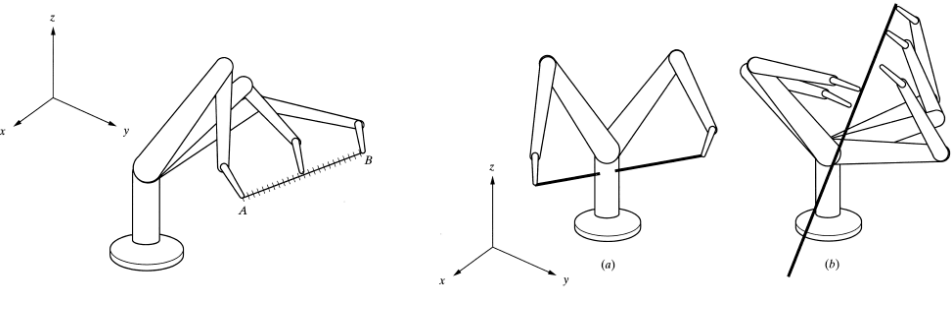
\includegraphics[scale=0.15]{graphics/trajectory.png}
        \end{figure}
        \column{.5\textwidth}
        \textbf{Operational space}
        \begin{itemize}
            \item path and motion is known
            \item easy to visualize
            \item prone to singlularities such as self-collision and sudden change in joint angles
            \item calculate complete path
            \item discretize path
            \item solve IK for each point
            \item can deal with obstacles
            \item Computationally expensive
        \end{itemize}
    \end{columns}   
\end{frame}

%%%%%%%%%%%%%%%%%%%%%%%%%%%%%%%%%%%%%%%%%%%%%%%%%%%%%%%%%%%%%%%%%%%%%%%%%%%%%%%%%%%%%%%%%%%%%%%%%%%%%%%%%

\begin{frame}{Robotics Lab}
    \begin{itemize}
        \item Tracking system 
        \item Robot
        \begin{itemize}
            \item Mobile platform
            \item Two 6 or 7 DoF manipulators
            \item Endeffector (gripper)
            \item Camera system for visaul feedback 
        \end{itemize}
        \item Laboratory equipment
        \begin{itemize}
            \item measurements units
            \item heater/cooler
            \item centrifuge
            \item etc.
        \end{itemize}
    \end{itemize}        
\end{frame}

%%%%%%%%%%%%%%%%%%%%%%%%%%%%%%%%%%%%%%%%%%%%%%%%%%%%%%%%%%%%%%%%%%%%%%%%%%%%%%%%%%%%%%%%%%%%%%%%%%%%%%%%%

\section{Task planning}
\begin{frame}{Task planning}
    \begin{itemize}
        \item tasks are a confined series of goals
        \item task planning needs feedback about the enviroment and status to react to disturbances
        \item a task can be defined and planned offline, but most likely needs to be adapted online
        % \item eg activity on edge (AOE)
        \item In the context of an autonomous biolab most tasks involve fluid handling in some sense leading to the basis problem of sloshing
    \end{itemize}
\end{frame}

%%%%%%%%%%%%%%%%%%%%%%%%%%%%%%%%%%%%%%%%%%%%%%%%%%%%%%%%%%%%%%%%%%%%%%%%%%%%%%%%%%%%%%%%%%%%%%%%%%%%%%%%%

\section{Sloshing Problem }
\begin{frame}{Sloshing Problem}
    \begin{columns}
        \column{.5\textwidth}
        \begin{itemize}
            \item occurs in partially filled containers subjected to external forces
            \item can cause spillage or force slow movements
            \item supression by feedforward control already tested by Reinhold et al. (2019)
            \item Obtaining measurements for feedback control is challenging
        \end{itemize}        
        \column{.5\textwidth}
        2
     
    \end{columns}   
\end{frame}

%%%%%%%%%%%%%%%%%%%%%%%%%%%%%%%%%%%%%%%%%%%%%%%%%%%%%%%%%%%%%%%%%%%%%%%%%%%%%%%%%%%%%%%%%%%%%%%%%%%%%%%%%

\begin{frame}{Modeling of liquid dynamics}
    \begin{columns}
        \column{.5\textwidth}
        \begin{itemize}
            \item linearized Navier-Stokes equations  
            \item superposition of j different modes
            \item each mode is described by a natural frequency $\omega_j$ 
            \item damping ratio is described by empirical relationships

        \end{itemize}        
        \column{.5\textwidth}

            \begin{equation} 
                \omega_{nj} = \sqrt{\frac{g \xi_j}{R} \tanh\left(\frac{h \xi_j}{R}\right)}
            \end{equation}

            \begin{equation}
                \delta_j = \frac{2.89}{pi}\sqrt{\frac{\nu}{\sqrt{R^3g}}}\left[1 + \frac{0.318}{\sinh\left(\frac{1.84h}{R}\right)}\frac{1-\frac{h}{R}}{\cosh\left(\frac{1.84h}{R}\right)}\right]
            \end{equation}
    \end{columns}   
\end{frame}

%%%%%%%%%%%%%%%%%%%%%%%%%%%%%%%%%%%%%%%%%%%%%%%%%%%%%%%%%%%%%%%%%%%%%%%%%%%%%%%%%%%%%%%%%%%%%%%%%%%%%%%%%

\begin{frame}{Simplifications}
    \begin{columns}
        \column{.5\textwidth}
        \begin{itemize}
            \item equivalent pendulum modeling
            \item relations between physical parameters and mode characteristics yield
            \begin{itemize}
                \item pivot points near surface
                \item first asymmetric mode is dominant
                \item pendulum orthogonal to surface
                \item planar surface
            \end{itemize} 
            \item excitation happens at the pivot point
        \end{itemize}        
        \column{.5\textwidth}
        \begin{figure}
            \centering
            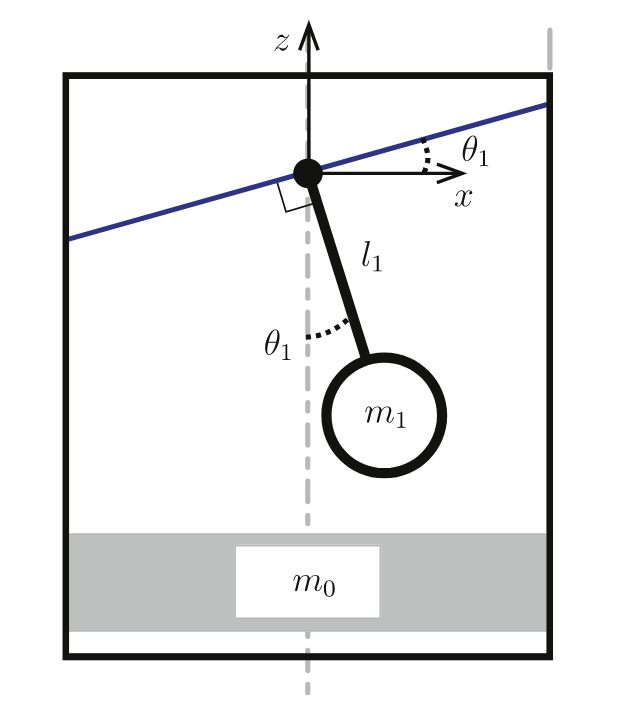
\includegraphics[scale=0.23]{graphics/sloshing_pendulum_simplified.png}
        \end{figure}
    \end{columns}   
\end{frame}

%%%%%%%%%%%%%%%%%%%%%%%%%%%%%%%%%%%%%%%%%%%%%%%%%%%%%%%%%%%%%%%%%%%%%%%%%%%%%%%%%%%%%%%%%%%%%%%%%%%%%%%%%

\begin{frame}{Modeling as pendulum on a (mobile) plane}
    \begin{columns}
        \column{.5\textwidth}
        \begin{itemize}
            \item earth bound sperical coordinate system 
            \item pendulum attachment point distance to plates COG is constant
            \item forces acting on the attachment point are directly correlated to the forces acting on the plate via the lever arms
            \item sloshing dynamics are described in the body frame around the pivot point 
            \item liquid behaviour is approximated as a pendulum
        \end{itemize}        
        \column{.5\textwidth}
            \begin{itemize}
                \item
            \end{itemize}
    \end{columns}   
\end{frame}



%%%%%%%%%%%%%%%%%%%%%%%%%%%%%%%%%%%%%%%%%%%%%%%%%%%%%%%%%%%%%%%%%%%%%%%%%%%%%%%%%%%%%%%%%%%%%%%%%%%%%%%%%

\begin{frame}{Modeling of sloshing}
    \begin{columns}
        \column{.5\textwidth}
        \begin{itemize}
            \item 
        \end{itemize}        
        \column{.5\textwidth}
            \begin{itemize}
                \item unforced dampened pendulum:
                
                \begin{equation}
                \ddot \theta = - \delta - \frac{g}{l} sin(\theta)    
                \end{equation}
                \begin{equation}
                    \dot \theta_1 = \theta_2
                \end{equation}
                \begin{equation}    
                    \dot \theta_2 = -\delta_3 \dot \theta_1^3 - \delta \dot \theta_1 + \frac{1}{l}[-gR(\theta_1) + A(t)] - [a(\frac{\theta}{\theta_{crit}})^b + c(\frac{\theta}{\theta_{crit}})^2d \dot \theta_1^m]
                \end{equation}
                \begin{equation}
                    A(t) = -x_0 \omega^2 sin(\omega t) 
                \end{equation}
            \end{itemize}
    \end{columns}   
\end{frame}

%%%%%%%%%%%%%%%%%%%%%%%%%%%%%%%%%%%%%%%%%%%%%%%%%%%%%%%%%%%%%%%%%%%%%%%%%%%%%%%%%%%%%%%%%%%%%%%%%%%%%%%%%

\end{document}